\documentclass[tikz,border=2pt]{standalone}
\usepackage{amsmath}
\usetikzlibrary{arrows.meta}
\begin{document}
% Entry game, payoffs (entrant, incumbent): Out (0,2); In then Accommodate (1,1) or Fight (-1,-1).
% At the incumbent's node Accommodate gives 1 > -1, so Fight is not sequentially rational even though
% (Out, Fight) is a Nash equilibrium; only (In, Accommodate) is sequentially rational for both.
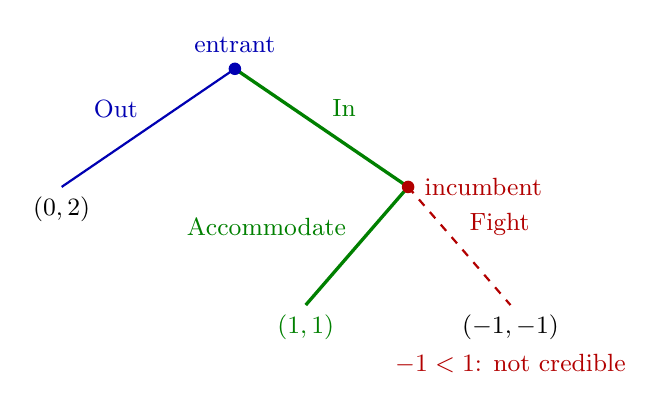
\begin{tikzpicture}[font=\small, >={Latex[length=2mm]},
    dec/.style={circle, fill, inner sep=1.6pt}]
  % edges
  \draw[thick, blue!70!black] (0,0) -- node[above left, pos=0.5] {Out} (-2.2,-1.5);
  \draw[very thick, green!50!black] (0,0) -- node[above right, pos=0.5] {In} (2.2,-1.5);
  \draw[very thick, green!50!black] (2.2,-1.5) -- node[above left, pos=0.5] {Accommodate} (0.9,-3);
  \draw[thick, red!70!black, dashed] (2.2,-1.5) -- node[above right, pos=0.5] {Fight} (3.5,-3);
  % nodes
  \node[dec, blue!70!black, label={[blue!70!black]above:entrant}] at (0,0) {};
  \node[dec, red!70!black, label={[red!70!black]right:incumbent}] at (2.2,-1.5) {};
  % leaves
  \node[anchor=north, inner sep=2pt] at (-2.2,-1.55) {$(0,2)$};
  \node[anchor=north, inner sep=2pt, green!50!black] at (0.9,-3.05) {$(1,1)$};
  \node[anchor=north, inner sep=2pt] at (3.5,-3.05) {$(-1,-1)$};
  \node[anchor=north, red!70!black] at (3.5,-3.5) {$-1<1$: not credible};
\end{tikzpicture}
\end{document}
